\documentclass[tikz,border=5pt]{standalone}
\usepackage{luatexja}
\usepackage[hiragino-pron]{luatexja-preset}
\usepackage{amsmath,amssymb}
\usepackage{pgfplots}
\pgfplotsset{compat=1.18}
\usetikzlibrary{arrows.meta,calc,decorations.markings,patterns,positioning}

% Common styles
\tikzset{
  axis/.style={-{Stealth[length=6pt]}, thick},
  curve/.style={thick, red},
  dashed curve/.style={thick, dashed, blue},
  dot/.style={circle, fill, inner sep=1.5pt},
  open dot/.style={circle, draw, fill=white, inner sep=1.5pt},
}

\begin{document}
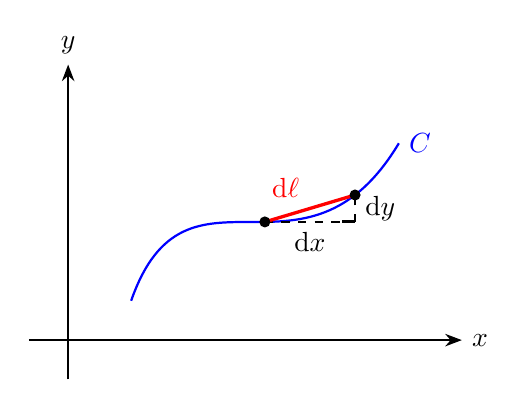
\begin{tikzpicture}[>=Stealth, thick]

  % Axes
  \draw[axis] (-0.5,0) -- (5,0) node[right] {$x$};
  \draw[axis] (0,-0.5) -- (0,3.5) node[above] {$y$};

  % Curve C — extract two points on the curve
  \draw[thick, blue]
    (0.8,0.5) .. controls (1.5,2.5) and (3,0.5) ..
    coordinate[pos=0.55] (P) coordinate[pos=0.85] (R) (4.2,2.5)
    node[right] {$C$};

  % Q = same x as R, same y as P (right-angle corner)
  \path let \p1 = ($(R)-(P)$) in coordinate (Q) at ([shift={(\x1,0)}]P);

  % dx, dy (black dashed)
  \draw[thick, dashed] (P) -- (Q) node[midway, below] {$\mathrm{d}x$};
  \draw[thick, dashed] (Q) -- (R) node[midway, right] {$\mathrm{d}y$};
  % dl (red, chord between two points on curve)
  \draw[very thick, red] (P) -- (R) node[midway, above left] {$\mathrm{d}\ell$};

  % Right angle mark
  \draw let \p1 = ($(R)-(P)$) in
    ([shift={(-0.15,0)}]Q) -- ++(0,{sign(\y1)*0.15}) -- ++(0.15,0);

  % Dots on curve
  \fill (P) circle (2pt);
  \fill (R) circle (2pt);

\end{tikzpicture}
\end{document}
